As we have seen the pair $C^1([0,T])\times C([0,T]) \ni z=(x^*,u^*): \mathbb{R_+}\ni t \mapsto \left(\frac{M}{2}, \frac{rM}{4}\right)$, is a stationary point, for the harvested fish functional, given a time horizon $T$. 

Since the initial populations can be different from the stationary point, i.e. $x_0\neq\frac{M}{2}$, we would like to implement an efficient strategy of harvesting, when we start from different initial conditions.

We propose as strategy the pair $(\hat{x}, \hat{u})$ close to the ideal dynamic $(x^*, u^*)$. In order to do a comparison between the distance of two different pairs, we propose the $\LL$ norm, i.e. 

\begin{align}
	\norm{\cdot}_{\LL([0,T])}:& \LL([0,T])\times \LL([0,T])\rightarrow \mathbb{R_+}\\
	:& (x, u)\mapsto \int_{0}^T x^2(t)\diff{t} +\int_{0}^T u^2(t)\diff{t}	
\end{align}. 

Using this norm as a measure of distance between functions, has all the properties of a norm, it is Fr\'echet differentiable and convex. It also has as advantage, that the functions belonging to this space form a Hilbert Space giving us a geometry for the space and reflexivity of the dual. All of them great advantages at the moment of implementing algorithms and developing theory for the process of finding optimal solutions of subsets in this spaces.


Consider the transformation $h=\frac{rM}{4}-u$, then equation \ref{eq: HarvestOpenLoop} transform into,
\begin{align}
\begin{array}{ll}
	\dev{x}{t}&=rx\left(1-\frac{x}{M}\right)-\frac{rM}{4}+h(t) \\
	x(0)&=x_0
\end{array}
 \label{eq: ConstrainOpenLoop}
\end{align}

We see, $h \rightarrow 0$ if, and only if $u\rightarrow \frac{rM}{4}$, under the $\LL$-norm.\footnote{In general in any $\mathrm{L}^p$ space.}.  Therefore, we would like to know the pair $(x^*, h^*)$, subject to the constraining equations \ref{eq: ConstrainOpenLoop}, such that the distance $\delta$, between itself and the optimal ideal pair for the harvested fish, i.e. $\left(\frac{M}{2}, 0\right)$, is the smallest possible among all the feasible pairs. i.e. 
\begin{equation}
\delta=	\norm{\left(\begin{array}{c}
			x^* \\ h^*
		\end{array}\right)-\left(\begin{array}{c} \frac{M}{2}\\ 0\end{array}\right)}_{\LL([0,T])}=\norm{x^*-\frac{M}{2}}_{\LL([0,T])}+\norm{h^*}_{\LL([0,T])}
\end{equation}

Could be useful to manipulate the strategy, in order to give more priority either to get closer to the optimal harvest rate or closer to the optimal population. Therefore, we add a term $\eta$ to the control to manipulate this desired ``priority''. 

Also it is necessary to add a penalty for the functions, that after a greedy extraction get further from the stationary population in a given time horizon $T$. By the previous requirements we propose as a fishing strategy the control that minimizes the following  functional,
\begin{equation}
\mathcal{J}(x,u)=\frac{1}{2} \left(x(T)-\frac{M}{2}\right)^2+\frac{1}{2}\norm{x-\frac{M}{2}}^2_{\LL([0,T])}+\frac{\eta}{2}\norm{h}^2_{\LL([0,T])}
\end{equation}

Since the operator $e:(x,h)\mapsto\dev{}{t}x-rx(1-x/M)-h$ is continuous Fr\'echet differentiable, by the implicit function theorem, $e(x,h)=0$ has solution. And $\mathcal{J}$ is convex and lower-semicontinuous. Hence the existence and uniqueness of the optimal is the minimizer is assured.\footnote{Add Hinze's Bibliography here.}

To solve this problem we will use an approach, first optimize then discretize. Which consists on finding analytically an expression that should be satisfied for infinite dimensional problem and then solve for it using a discrete numerical method, one advantage of this approach is that the solution found by the numerical method carry only the uncertainties proper of the implemented method. 


By the structure of the problem we can apply the Pontryagin's Theorem, in order to find the expression for the minimizer element.

That is, if $U$ is the set of values of permissible controls then the states that the optimal control $h^∗$ must satisfy:
\begin{equation}
H\left( x^*, u^*, \lambda^*, t \right) \leq H(x^*,u, \lambda^*, t), \qquad \forall u \in U,\, t \in [0, T]	\label{eq: HamiltonianOptimalCondition.}
\end{equation}	
where $x^* \in C^1[0, T]$ is the optimal state trajectory and $\lambda^* \in \mathrm{BV}[0, T]$ is the optimal costate trajectory. With the proper Hamiltonian for this problem,

\begin{equation}
H\left( x, u, \lambda, t \right)=\lambda\left(	rx\left(1-\frac{x}{M}\right)-\frac{rM}{4}+h\right)+\frac{1}{2}\left(x-\frac{M}{2}\right)^2+\frac{\eta}{2}h^2
\end{equation}

We see that this Hamiltonian is well defined since, our solution should satisfy $e(x,h)=0$, and the penalty imposed is consistent with the shape of the Hamiltonian.
\begin{equation}
	H\left(x(T), h(T), \lambda(T), T \right)=\Upsilon(x(T))=\frac{1}{2}\left(x(T)-\frac{M}{2}\right)^2
\end{equation}
Therefore, the tuple $(x^*, h^*,\lambda^*)$, should satisfy the necessary conditions,
\begin{align}
\begin{array}{ll}
\dev{}{t}\left(\lambda^*\right)&=-\pdev{H}{x^*} \\
\lambda^*(T)&=\left.\dev{\Upsilon}{x}\right|_{x^*=x(T)}
\end{array}
\end{align}
and,
\begin{align}
\pdev{H}{h^*}=0
\end{align}
By the above equations our problem is reduce to find the solutions to,
\begin{equation}
\begin{array}{ll}
\dev{}{t}\left(\lambda^*\right)&=-r\lambda^*+\frac{2r}{M}x^*\lambda^* -x^*+\frac{M}{2} \\
\lambda^*(T)&=x^*(T)-\frac{M}{2}
\end{array}	
\end{equation}
and
\begin{align}
	0&=\lambda + \eta h \\
	\implies&\lambda=-\eta h
\end{align}
Therefore, we need to solve the system of equations
\begin{align}
\dev{}{t}\left(\begin{array}{l}
\lambda^*\\x^*
\end{array}\right)&= \left(\begin{array}{l}
-r\lambda^*+\frac{2r}{M}x^*\lambda^*-x^*+\frac{M}{2}\\rx^*\left(1-\frac{1}{M}x^*\right)-\frac{rM}{4}-\frac{1}{\eta} \lambda(t)
\end{array}\right)\label{eq: PontryaginLambdaCondition}\\
\lambda^*(T)&=x^*(T)-M/2\label{eq:PontryaginBoundary}\\
x^*(0)&=x_0 \label{eq:Pontryaginx0}
\end{align}

In order to implement the discrete solution, we need to  of the above expression, we propose a Foward-Backward-Method, starting for some $x^{[0]}$, $\lambda^{[0]}$, we construct a sequence $\left(x^{[n]}, \lambda^{[n]}\right)_{n\in \mathbb{N}}$solve iteratively for,
\begin{align}
	\dev{}{t}\left(\begin{array}{l}
	\lambda^{[n+1]}\\x^{[n+1]}
	\end{array}\right)&= \left(\begin{array}{l}
	-r\lambda^{[n+1]}+x^{[n+1]}\lambda^{[n+1]} \frac{2r}{M}-x^{[n+1]}+\frac{M}{2}\\rx^{[n+1]}\left(1-\frac{1}{M}x^{[n+1]}\right)-\frac{rM}{4}-\frac{1}{\eta} \lambda^{[n]}(t)
	\end{array}\right)\label{eq: FBS}\\
	\lambda^{[n+1]}(T)&=x^{[n+1]}(T)-M/2\label{eq: FBSBoundary}\\
	x^{[n+1]}(0)&=x_0 
\end{align}
And after each iteration we substitute the value of 
$\lambda^{[n+1]}\leftarrow0.5\lambda^{[n+1]}+0.5 \lambda^{[n]}$. 

The idea is that after many iterations the contributions of the initials conditions are getting exponentially less significant, and the converging value of $\lambda^*$ is solution for the equations\ref{eq:PontryaginBoundary}, \ref{eq: PontryaginLambdaCondition} and \ref{eq:Pontryaginx0}.
We present, the result of executing the above algorithm for,
$T=12$, $\eta=20.0$, $M=780500$, $r=0.8$, and $x_0=0.45M$.
\begin{figure}[H]
	\caption{Smooth Control for Open Loop Strategy.}
	\begin{subfigure}{0.48\textwidth}
		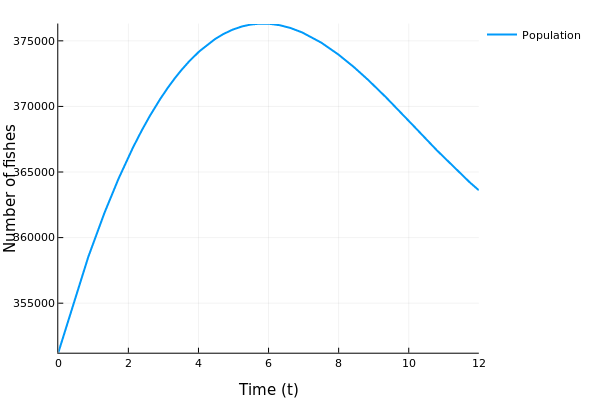
\includegraphics[width=0.95\textwidth]{Population.png}
		\caption{Population under open loop control.}
	\end{subfigure}
	\begin{subfigure}{0.48\textwidth}
		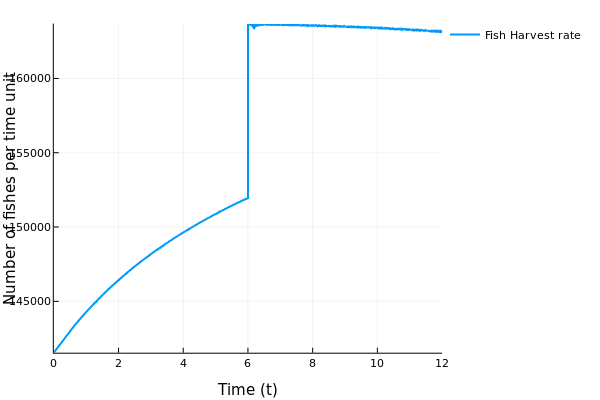
\includegraphics[width=0.95\textwidth]{Harvest}
		\caption{Harvest rate solution for \ref{eq: PontryaginLambdaCondition} }
	\end{subfigure}
\end{figure}
Under the above conditions, the harvested population is given by $\int_{0}^{T} u(t) \diff{t} \approx 1.8670261\times 10^6$, in contrast with the optimal $J^*(\frac{M}{2}, \frac{rM}{4})=\frac{rM}{4}T\approx1.8732\times 10^6$.
%\begin{equation}
%\Min{\substack{x\in X \\ u \in U}}{\mathcal J(x,u)}
%\end{equation}
%subject to,
%\begin{equation}
%	e(x,u)=0
%\end{equation}
